\documentclass[10pt,xcolor=table]{beamer}
\usetheme{Warsaw}
\usecolortheme{dolphin}
\usepackage[utf8]{inputenc}
\usepackage[spanish,es-nodecimaldot]{babel}
\usepackage{amsmath}
\usepackage{amsfonts}
\usepackage{amssymb}
\usepackage{graphicx}
\usepackage{multimedia}
\usepackage{booktabs}
\usepackage{physics}
\author[Cindy Castell\'on]{{\footnotesize Presentado por}\\  \vspace{0.15 cm}
	Cindy Mariella Castellón Salguero\\
	\vspace{0.3 cm}
	{\footnotesize Asesorado por}\\ \vspace{0.15 cm}
	Ph. D. Hermes Le\'on Vargas \\ \vspace{0.15 cm}
	M. Sc. Ra\'ul Antonio Henr\'iquez Ort\'iz \vspace{0.4 cm}}
	
\title[Estudio de la componente mu\'onica de cascadas atmosf\'ericas]{{\normalsize Trabajo de graduaci\'on:} \\ \vspace{0.5 cm}
\textbf{\textit{Estudio de la componente mu\'onica en la distribuci\'on lateral de cascadas atmosf\'ericas}}}
%\setbeamercovered{transparent} 
\setbeamertemplate{headline}{}
\setbeamertemplate{navigation symbols}{} 
\setbeamertemplate{footline}{}
% set the footline
\setbeamertemplate{footline}{
  \hbox{%
% left block with the shortname, it is set in the \author command
    \begin{beamercolorbox}[wd=.30\paperwidth,ht=2.25ex,dp=1ex,center]%
      {author in head/foot}%
      \usebeamerfont{author in head/foot}\insertshortauthor
    \end{beamercolorbox}%
% center block with the short title, it is set in the \title command
    \begin{beamercolorbox}[wd=.60\paperwidth,ht=2.25ex,dp=1ex,center]%
      {title in head/foot}%
      \usebeamerfont{title in head/foot}\insertshorttitle
    \end{beamercolorbox}%
% right block with the number of slides
    \begin{beamercolorbox}[wd=.10\paperwidth,ht=2.25ex,dp=1ex,right]%
      {date in head/foot}%
      \usebeamerfont{date in head/foot}
      \insertframenumber{} / \inserttotalframenumber\hspace*{1em}
    \end{beamercolorbox}}%
  \vskip0pt%
}

\makeatletter
\setbeamertemplate{frametitle}{%
  \nointerlineskip%
  \vskip-2pt%
  \hbox{\leavevmode
    \advance\beamer@leftmargin by -12bp%
    \advance\beamer@rightmargin by -12bp%
    \beamer@tempdim=\textwidth%
    \advance\beamer@tempdim by \beamer@leftmargin%
    \advance\beamer@tempdim by \beamer@rightmargin%
    \hskip-\Gm@lmargin\hbox{%
      \setbox\beamer@tempbox=\hbox{\begin{minipage}[b]{\paperwidth}%
          \vbox{}\vskip-.75ex%
          \vspace{0.14cm}% <- change here to whatever you want
          \leftskip0.3cm%
          \rightskip0.3cm plus1fil\leavevmode
          \usebeamercolor[fg]{frametitle}\usebeamerfont{frametitle}\strut\insertframetitle\strut\par%
          \ifx\insertframesubtitle\@empty\else%
            {\usebeamerfont*{framesubtitle}{\usebeamercolor[fg]{framesubtitle}\insertframesubtitle}\strut\par}%
          \fi%
          \nointerlineskip
          \vspace{0.1cm}
          \vbox{}%
          \end{minipage}}%
      \beamer@tempdim=\ht\beamer@tempbox%
      \advance\beamer@tempdim by 2pt%
      \begin{pgfpicture}{0pt}{0pt}{\paperwidth}{\beamer@tempdim}
        \usebeamercolor{frametitle right}
        \pgfpathrectangle{\pgfpointorigin}{\pgfpoint{\paperwidth}{\beamer@tempdim}}
        \pgfusepath{clip}
        \pgftext[left,base]{\pgfuseshading{beamer@frametitleshade}}
      \end{pgfpicture}
      \hskip-\paperwidth%
      \box\beamer@tempbox%
    }%
    \hskip-\Gm@rmargin%
  }%
  \nointerlineskip
    \vskip-0.2pt
    \hbox to\textwidth{\hskip-\Gm@lmargin\pgfuseshading{beamer@topshade}\hskip-\Gm@rmargin}
    \vskip-2pt
}

\mode<presentation> {
% coloring for slides other options: beetle, dove
  \usecolortheme{dolphin}
% to include a slide with the table of contents
 \AtBeginSection[] {
  \begin{frame}
    \tableofcontents[currentsection]
  \end{frame} }
}

%\logo{} 
\institute{Escuela de Física, Facultad de Ciencias Naturales y Matem\'atica \\ \vspace{0.15 cm}Universidad de El Salvador} 
\date{} 
\subject{Proyecto de investigación} 



\begin{document}

\begin{frame}
\titlepage
\end{frame}

\begin{frame}
\tableofcontents
\end{frame}

\section{Introducci\'on}
\begin{frame}{Rayos cósmicos}
	\begin{columns}
		\begin{column}{0.4\textwidth}
		Descubiertos por Victor Hess en 1912; los rayos c\'osmicos son partículas cargadas originadas en ambientes extremos del universo, que llegan a la Tierra con altas energías ($>10^9$ eV).
		\vspace{\fill}
		\end{column}
		\begin{column}{0.6\textwidth}
			\begin{figure}
			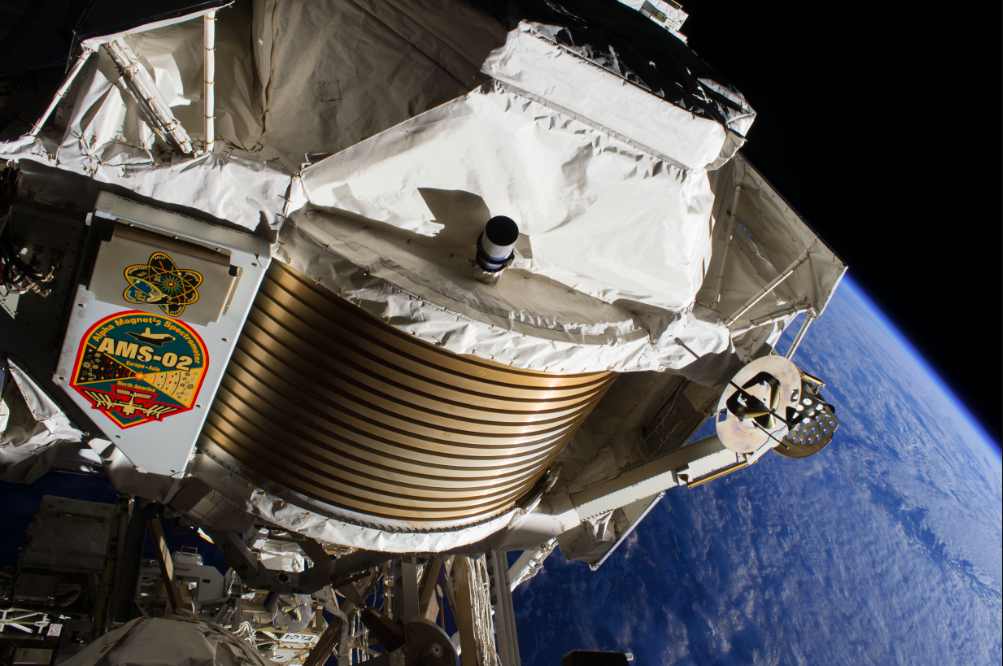
\includegraphics[width=0.75\textwidth]{Figuras/spacedetector} 
			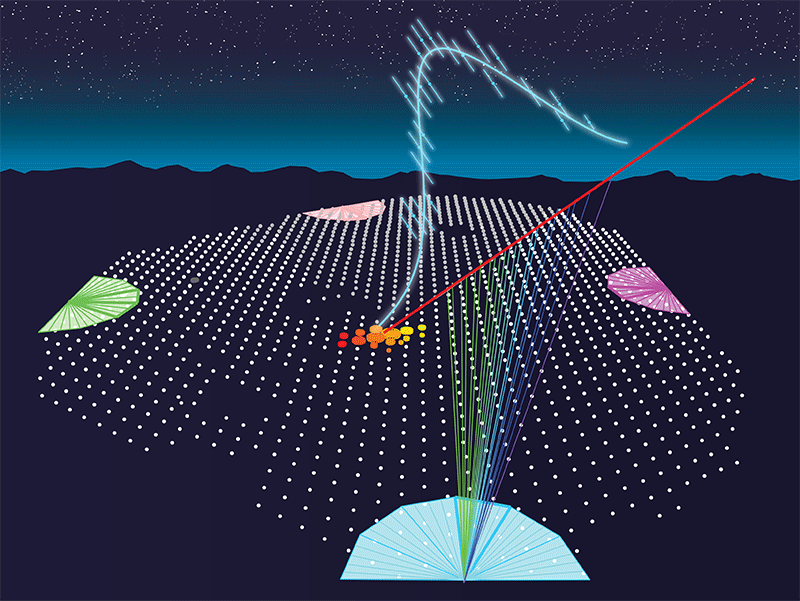
\includegraphics[width=0.75\textwidth]{Figuras/surfacedetector}
			\end{figure}				
		\end{column}			
	\end{columns}	
\end{frame}

%\begin{frame}
%\begin{columns}
%		\begin{column}{0.5\textwidth}
%		\center
%		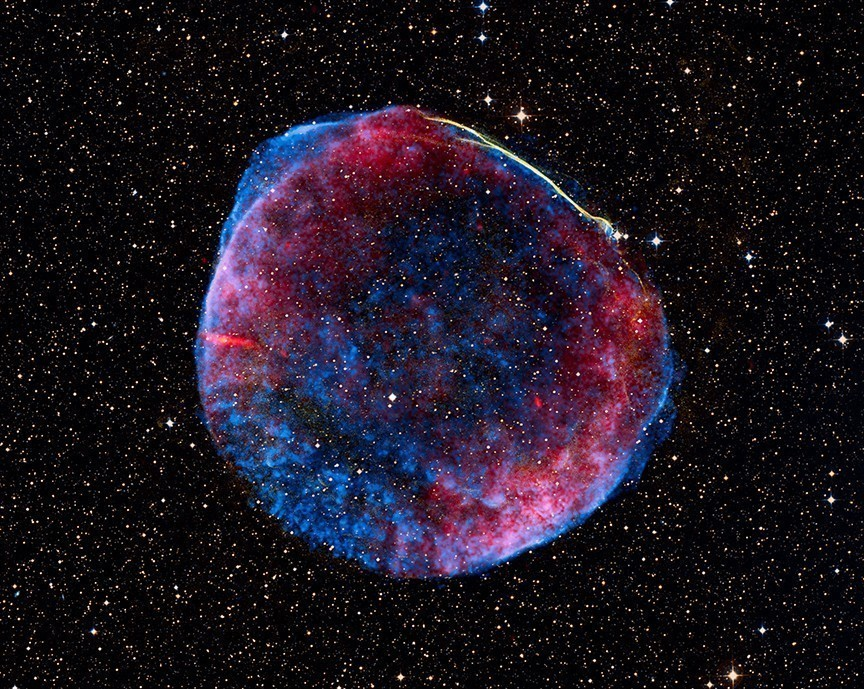
\includegraphics[width=1\textwidth, height=0.5\textheight]{Figuras/snr}
%		\end{column}
%		
%		\begin{column}{0.5\textwidth}
%		\center
%		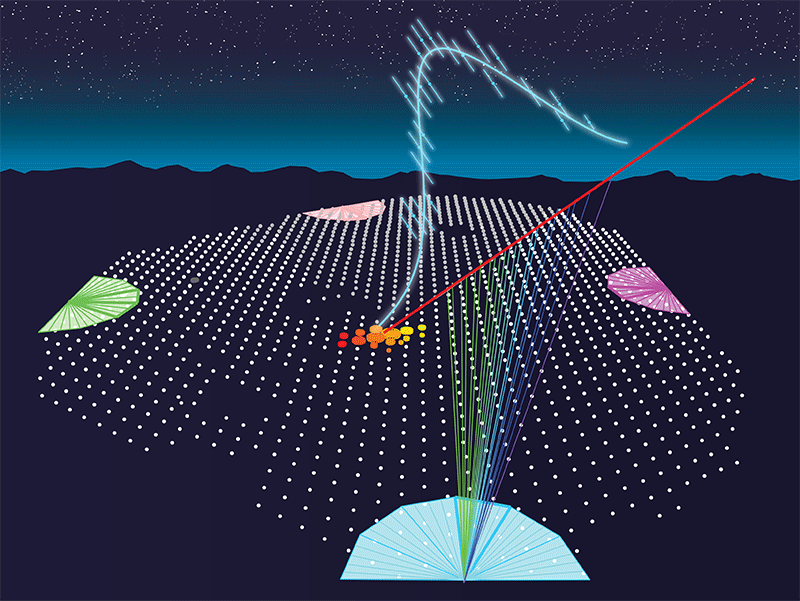
\includegraphics[width=1\textwidth, height=0.5\textheight]{Figuras/surfacedetector}
%		\end{column}
%\end{columns}
%\end{frame}

\begin{frame}{Cascadas Atmosf\'ericas}
	\begin{figure}
	\centering
	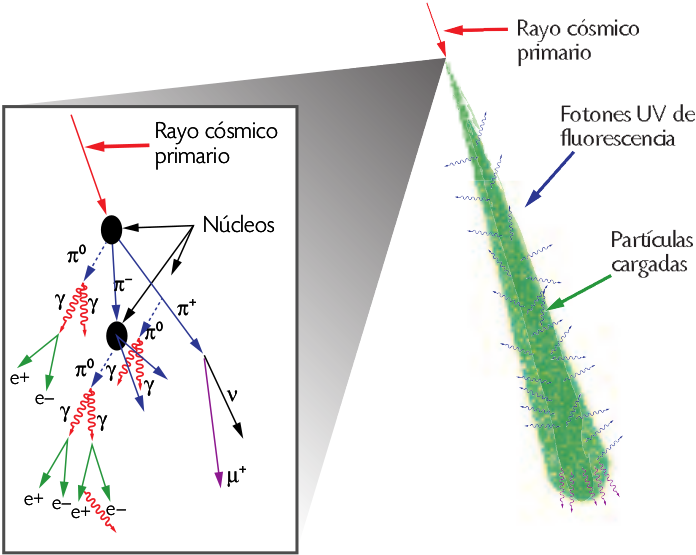
\includegraphics[width=0.75\textwidth]{Figuras/air_shower} 
	\caption{Esquema de formación y desarrollo de una cascada (Bahena, 2013).}
	\label{fig:airshower}
	\end{figure}	
\end{frame}	
	
\begin{frame}{Interacciones}
\vspace{\fill}
Los procesos m\'as relevantes para los rayos c\'osmicos en la atm\'osfera: \vspace{0.5 cm}
	\begin{columns}
		\begin{column}{0.5\textwidth}
			\begin{block}{Electrodin\'amicos}
				\begin{itemize}
				\item Producci\'on de pares.
				\item \textit{Bremsstrahlung}.
				\item Efecto fotoel\'ectrico.
				\item Efecto Compton.
				\end{itemize}
			\end{block}
		\end{column}
		\begin{column}{0.5\textwidth}
			\begin{block}{Hadr\'onicos}
			\vspace{0.225 cm}
				\begin{itemize}
				\item Colisiones hadr\'on - n\'ucleo.
				\item Reacciones fotonucleares.
				\item Fragmentaci\'on nuclear.
				\end{itemize}
			\vspace{0.255 cm}
			\end{block}
		\end{column}
	\end{columns}
	\vspace{0.5 cm}
	Adem\'as de decaimientos y procesos de propagaci\'on como ionizaci\'on del medio y dispersi\'on de Coulomb.
	\vspace{\fill}
\end{frame}

\begin{frame}{Muones en cascadas}
Los muones se producen principalmente en decaimiento de mesones: \vspace{0.5 cm}
	\begin{LARGE}
	\textcolor{blue} {
		\begin{align*}
		\pi^{\pm}	&\longrightarrow 	\mu^{\pm} + \nu_{\mu}(\bar{\nu}_{\mu})
		\end{align*}
		\begin{align*}
		K^{\pm}		&\longrightarrow 	\mu^{\pm} + \nu_{\mu}(\bar{\nu}_{\mu})
		\end{align*}
	}
	\end{LARGE}

%ideas: -muones vienen de decaimiento de mesones
%- numero de muones depende de E0 y de A
%-muones viven lo suficiente para ser detectados en el suelo
%- muones tienen cross section peque;a asi que no interactuan antes de llegar al suelo.
\end{frame}

\begin{frame}{HAWC}
\textit{The High-Altitude Water Cherenkov gamma-ray observatory} (HAWC), a 4100 m s. n. m, detecta part\'iculas producidas en cascadas atmosf\'ericas de energ\'ias entre 1 y 100 TeV. \vspace{0.3cm}
	\begin{columns}
		\begin{column}{0.7\textwidth}
		\center
		\href{run:Figuras/HAWC.mov?autostart&loop&start=2&stop=120}
       {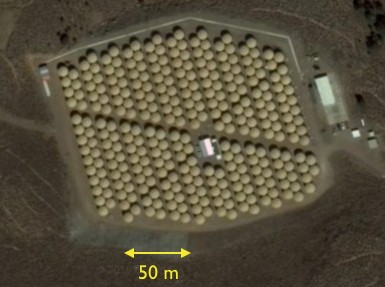
\includegraphics[width=1\textwidth]{Figuras/hawc-array}}
%		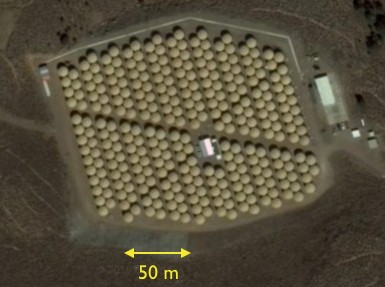
\includegraphics[width=1\textwidth]{Figuras/hawc-array}
		\end{column}
		
		\begin{column}{0.3\textwidth}
		\center
		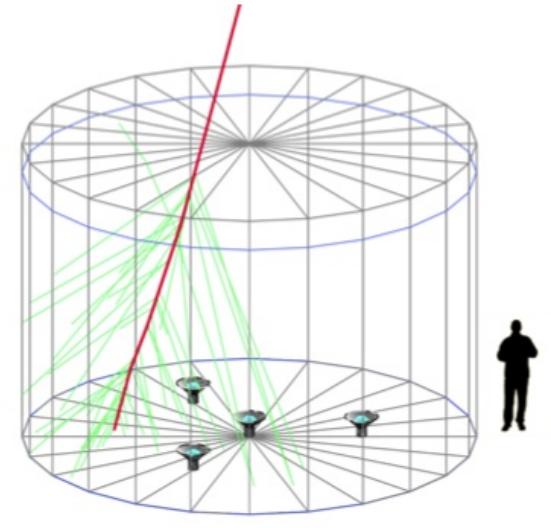
\includegraphics[width=0.9\textwidth]{Figuras/hawc-tank}
		(Figuras de la colaboraci\'on HAWC)
		\end{column}
	\end{columns}

%ideas - foto de hawc
%- rango de energias 1-100 TeV
%-detectan particulas por radiacion de cherenkov en el agua.
%- que se ha hecho con hawc: anisotropia, antiprotones y fuentes galacticas de RC.
\end{frame}
	
%	\begin{frame}{Modelos de chubascos}
%		\begin{block}{Sección eficaz}
%		Probabilidad de que una partícula interactúe.
%		\end{block}	
%		\vspace{5 mm}
%		\begin{block}{Multiplicidad}
%		Número de mesones producidos en una interacción hadrónica.
%		\end{block}	
%		\vspace{5 mm}
%		\begin{block}{Inelasticidad}
%		Fracción de la energía que se invierte en producción de mesones.
%		\end{block}			
%	\end{frame}		
	
\begin{frame}{Objetivos}
	\begin{block}{Objetivo general}
	Estudiar mediante simulaciones computacionales la distribución lateral de muones en cascadas atmosféricas con energías iniciales en el rango del observatorio HAWC (1-100 TeV).
	\end{block}
	\vspace{0.3 cm}
	\begin{block}{Objetivos espec\'ificos}
		\begin{enumerate}
		\item Caracterizar la densidad de muones a varias distancias del eje de la cascada atmosf\'erica en funci\'on de la energ\'ia inicial. \vspace{0.1 cm}
		\item Comparar las distribuciones de muones en cascadas atmosf\'ericas iniciadas por distintas part\'iculas primarias. \vspace{0.1 cm}
		\item Evaluar la influencia del modelo de interacciones hadr\'onicas de altas energ\'ias utilizado en las simulaciones sobre la distribuci\'on lateral de muones. \vspace{0.1 cm}
		\end{enumerate}
	\end{block}
\end{frame}

\section{Metodolog\'ia}
\begin{frame}{AIRES}
	\begin{columns}
		\begin{column}{0.5\textwidth}
		Para las simulaciones se utiliz\'o el sistema AIRES (AIR shower Extended Simulations) (Sciutto, 2001), dise\~{n}ado para simular cascadas atmosf\'ericas realistas, que incluye los principales paquetes de interacciones hadr\'onicas de altas energ\'ias actualizados.\\
		\end{column}
		\begin{column}{0.5\textwidth}
			\begin{center}
				\begin{figure}
				\fbox{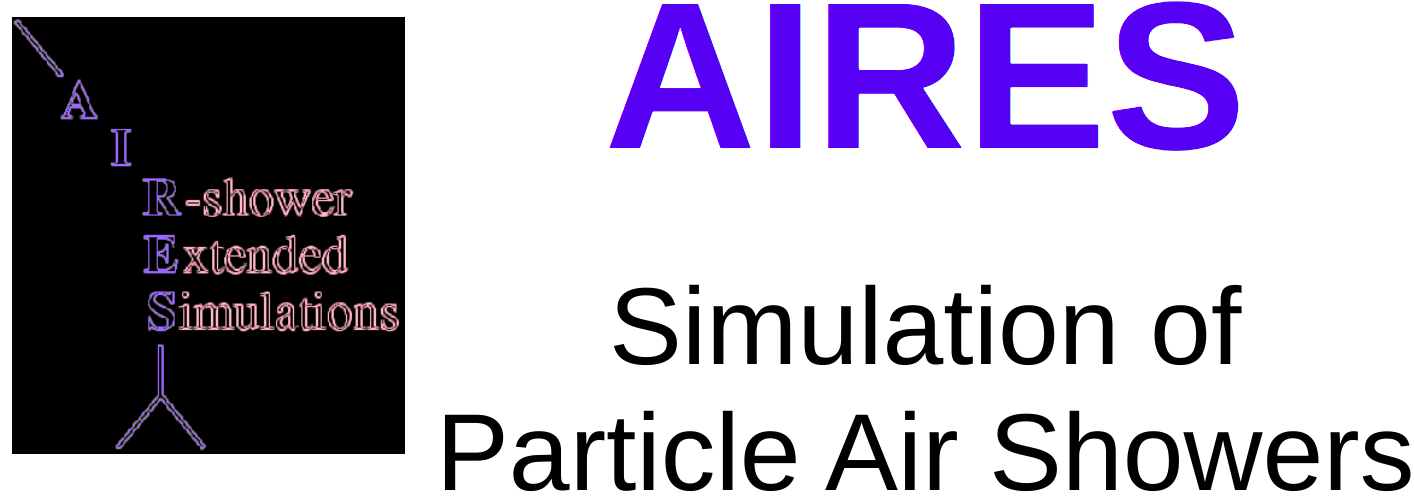
\includegraphics[width=\textwidth]{Figuras/aires_logo}}
				\caption{{\footnotesize AIRES es desarrollado en el Departamento de F\'isica de la Universidad Nacional de La Plata, Argentina. Disponible en \url{http://aires.fisica.unlp.edu.ar/}.}}
				\end{figure}
			\end{center}
		\end{column}	
	
	\end{columns}
\end{frame}

\begin{frame}{Simulaciones de cascadas}
Con cada uno de los tres modelos de interacciones hadrónicas de altas energías (Sibyll 2.3d, EPOS-LHC y QGSJETII-04) se simularon 20,000 eventos en la ubicaci\'on  del observatorio HAWC, ubicado en Puebla, M\'exico, con latitud de 19$^{o}$ y altura de 4100 m sobre el nivel del mar. \\
	\begin{columns}
		\begin{column}{0.5\textwidth}
			\begin{table}[]
			\caption{Especificaciones de entrada.}
				\begin{tabular}{@{}cl@{}}
				{\color[HTML]{0E3EF0} Part\'icula} & p, Fe      		\\ \midrule
				{\color[HTML]{0E3EF0} $E_0$}       & $1-100$ TeV  	\\ \midrule
				{\color[HTML]{0E3EF0} $\theta_0$}  & $0-45^{\circ}$	\\ \midrule
				{\color[HTML]{0E3EF0} $\phi_0$}    & $0-360^{\circ}$	\\ \midrule
				{\color[HTML]{0E3EF0} $E_{\mu}$}   & $> 1.60$ GeV 
				\end{tabular}
			\end{table}
		\end{column}
		
		\begin{column}{0.5\textwidth}
		\vspace{0.7cm}
			\begin{center}
			\begin{figure}
			\fbox{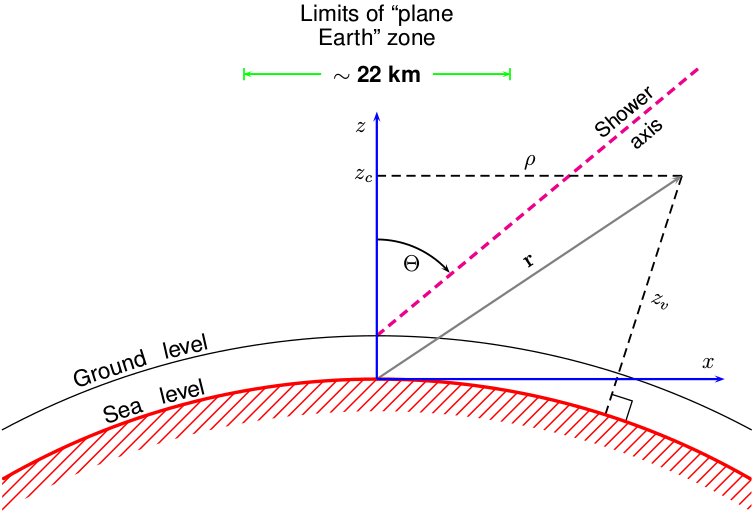
\includegraphics[width=0.8\textwidth]{Figuras/coordinates}}
			\caption{{\footnotesize Sistema de coordenadas en AIRES (Sciutto, 2001).}}
			\end{figure}
			\end{center}
		\end{column}
	
	\end{columns}
	
\end{frame}


\section{Resultados}
\begin{frame}{Distribuci\'on de muones}
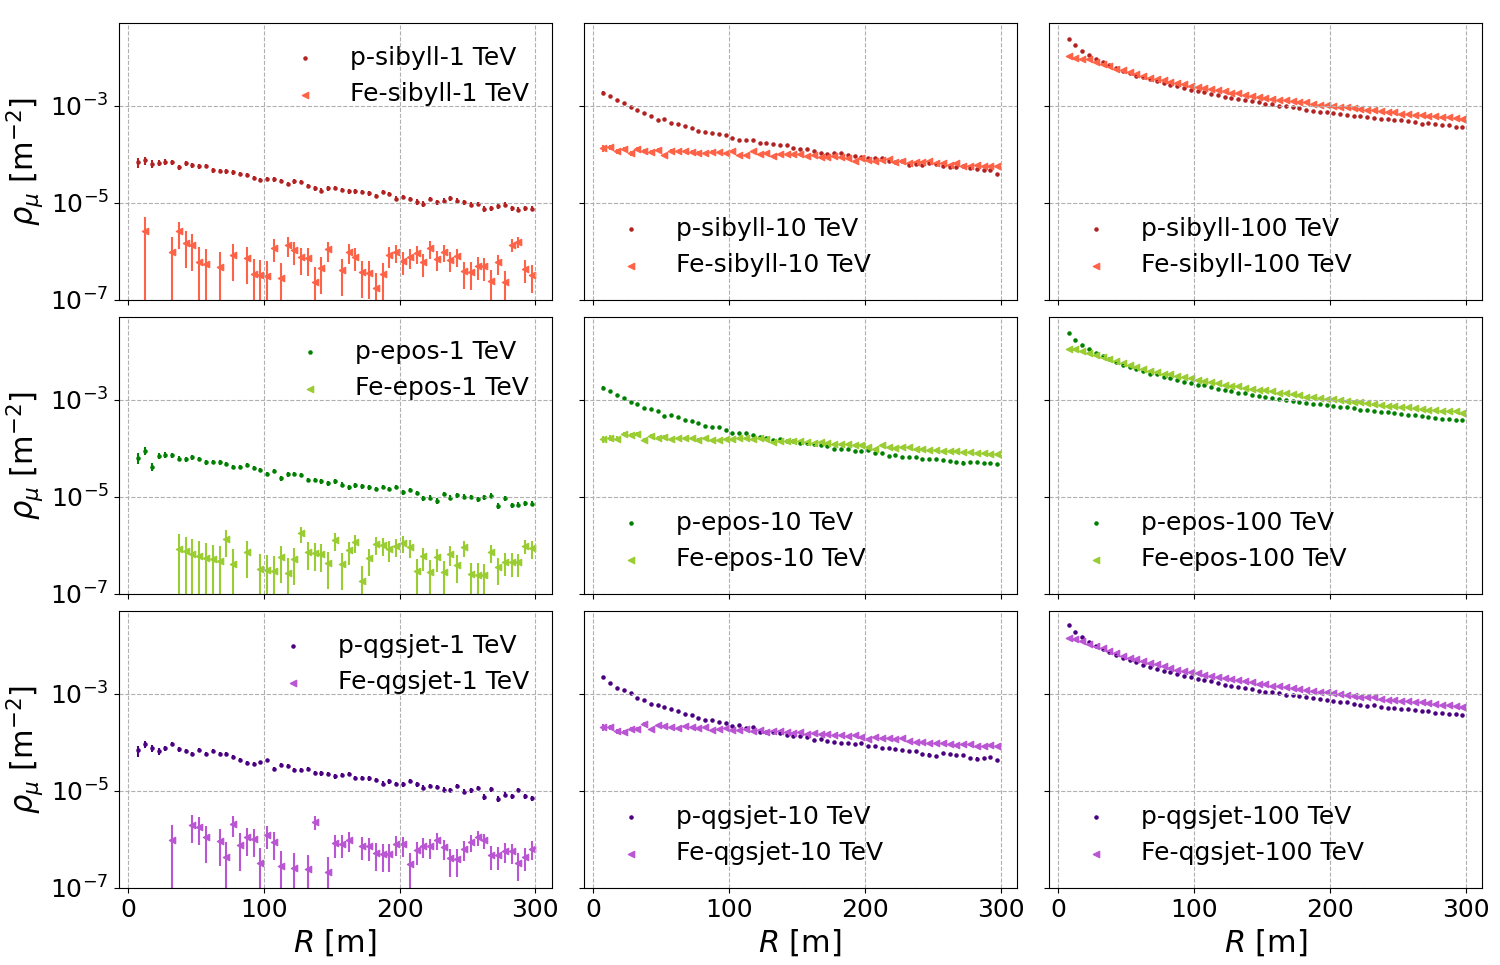
\includegraphics[width=\textwidth]{Figuras/lateraldist.png}
\end{frame}

\begin{frame}{Distribuci\'on de muones}
	\begin{columns}
		\begin{column}{0.5\textwidth}
		Cada distribuci\'on lateral de muones se ajust\'o a una funci\'on de la forma
				\begin{align*} 
				\rho_{\mu}(r) = A \qty(\frac{r}{r_M})^{s-3}\qty(1+\frac{r}{r_M})^{s-4.5},
				\end{align*}	
			utilizada usualmente para ajustar distribuciones de carga efectiva en HAWC, donde $r_M = 124.21$ (Malone, 2018).
		
		\end{column}
	
		\begin{column}{0.5\textwidth}
		\begin{overlayarea}{\textwidth}{0.8\textheight}
		\only<1>{
		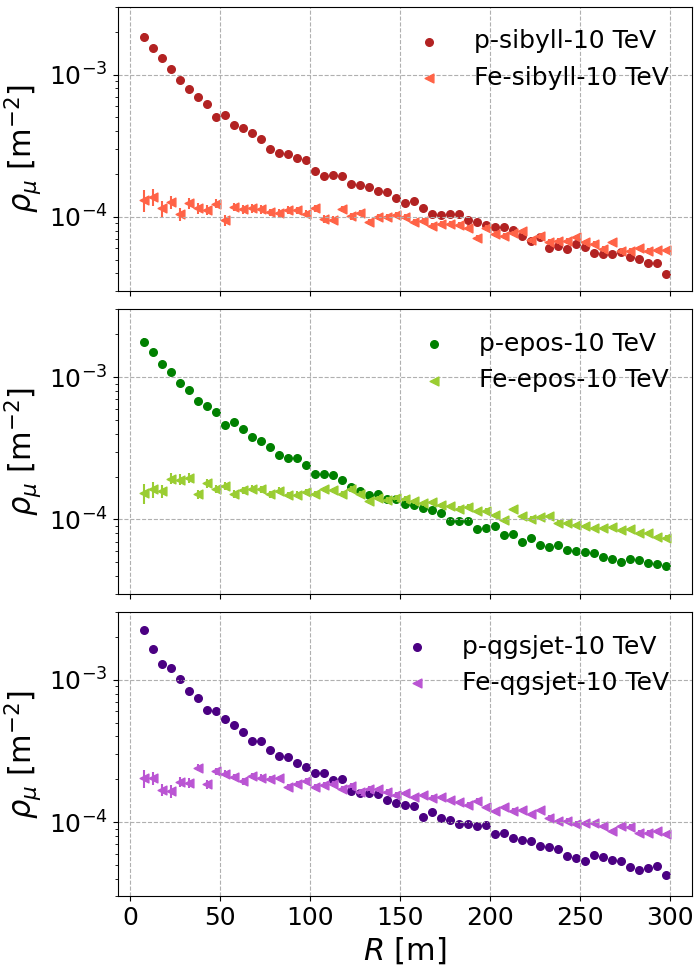
\includegraphics[width=1\textwidth]{Figuras/p-lateraldist10TeV.png}
		}
		\only<2>{
		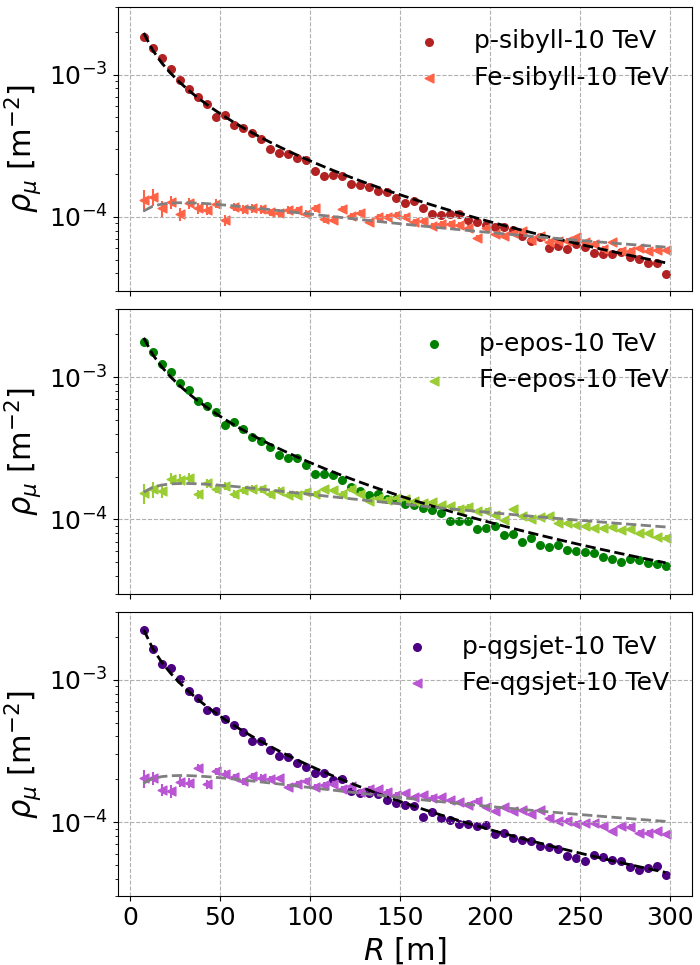
\includegraphics[width=1\textwidth]{Figuras/p-lateraldist10TeV-wfits.png}
		}
		\end{overlayarea}
		\end{column}
		
	\end{columns}
\end{frame}


%\begin{frame}{Distribuci\'on de muones}
%	\begin{columns}
%		\begin{column}{0.5\textwidth}
%		\onslide<1->{
%		Cada distribuci\'on lateral de muones se ajust\'o a una funci\'on de la forma
%			\begin{align*} 
%			\rho_{\mu}(r) = A \qty(\frac{r}{r_M})^{s-3}\qty(1+\frac{r}{r_M})^{s-4.5},
%			\end{align*}	
%		utilizada usualmente para ajustar distribuciones de carga efectiva en HAWC (Malone, 2018).}		
%		\end{column}
%		
%		\begin{column}{0.5\textwidth}
%		\center
%		\includegraphics<1>[width=1\textwidth]{Figuras/p-lateraldist10TeV.png}
%		\includegraphics<2>[width=1\textwidth]{Figuras/p-lateraldist10TeV-wfits.png}
%		\end{column}
%	\end{columns}
%\end{frame}
%
%\begin{frame}{Distribuci\'on de muones}
%	\begin{columns}
%		\begin{column}{0.5\textwidth}
%		Cada distribuci\'on lateral de muones se ajust\'o a una funci\'on de la forma
%			\begin{align*} 
%			\rho_{\mu}(r) = A \qty(\frac{r}{r_M})^{s-3}\qty(1+\frac{r}{r_M})^{s-4.5},
%			\end{align*}	
%		utilizada usualmente para ajustar distribuciones de carga efectiva en HAWC (Malone, 2018).			
%		\end{column}
%		
%		\begin{column}{0.5\textwidth}
%		\center
%		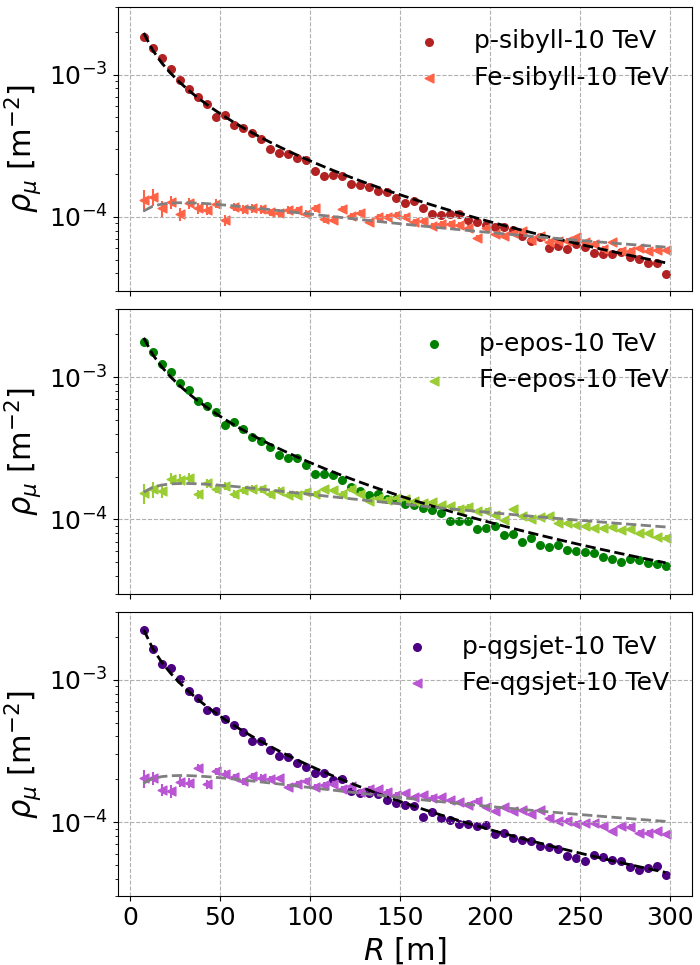
\includegraphics[width=1\textwidth]{Figuras/p-lateraldist10TeV-wfits.png}
%		\end{column}
%	\end{columns}
%\end{frame}



\begin{frame}{Modelos hadr\'onicos}
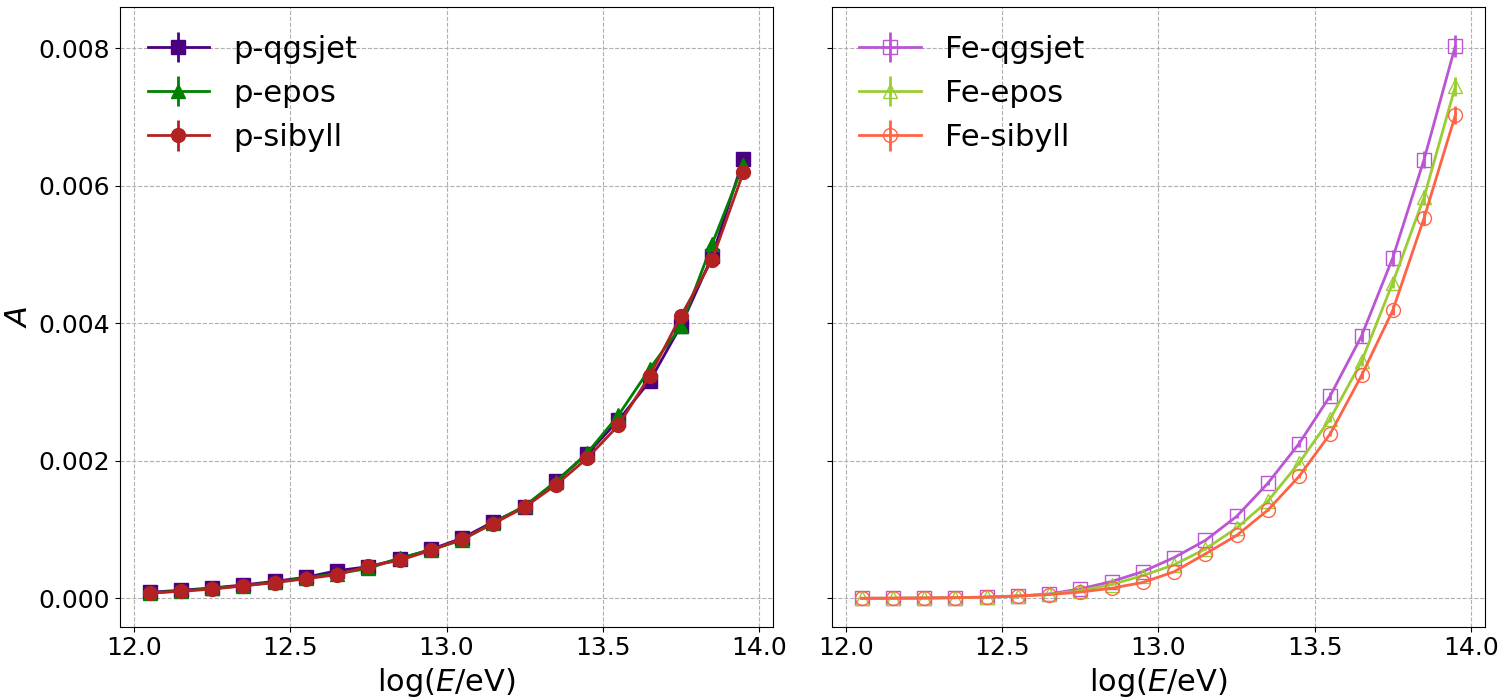
\includegraphics[width=\textwidth]{Figuras/p-models_nkgA.png}
\end{frame}

\begin{frame}{Modelos hadr\'onicos}
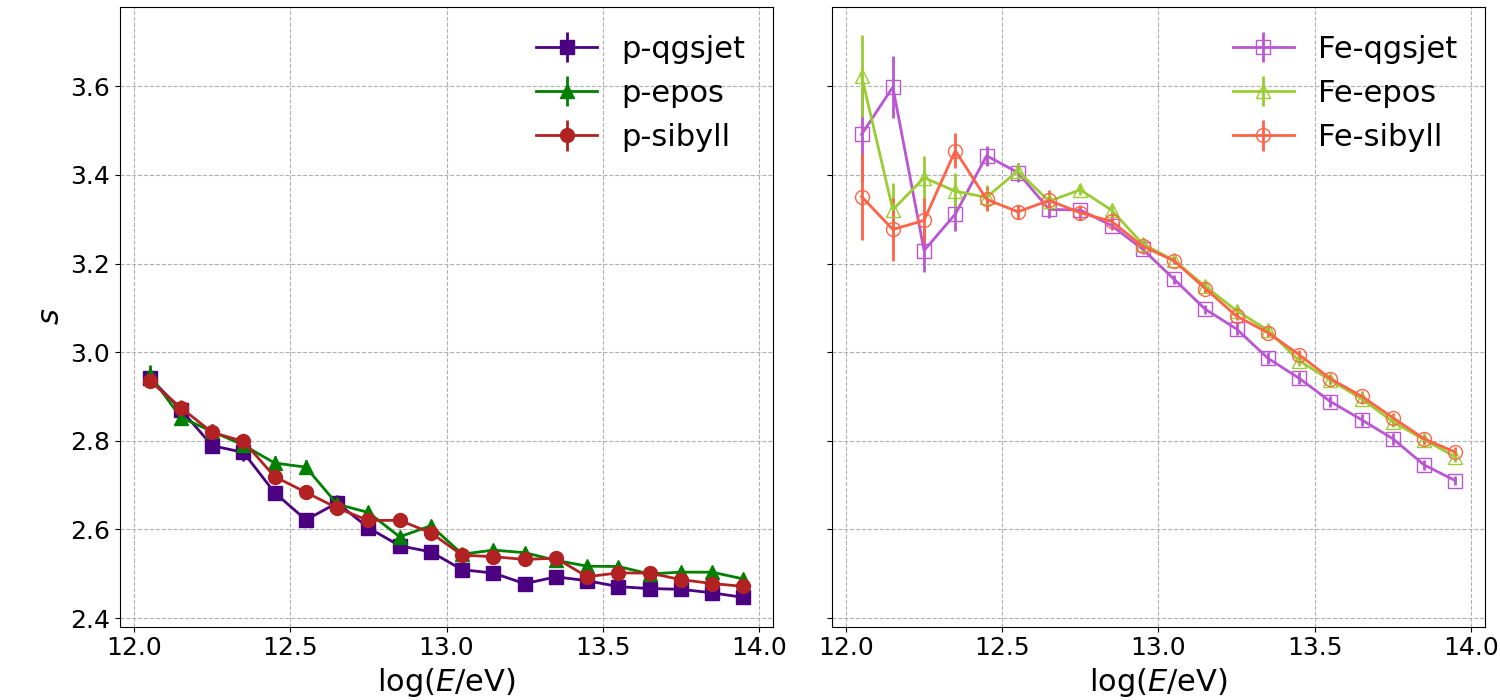
\includegraphics[width=\textwidth]{Figuras/p-models_nkgs.png}
\end{frame}

\begin{frame}{Part\'iculas primarias}
El modelo Heitler-Matthews (Matthews, 2005) utilizando un modelo de superposici\'on, predice un mayor n\'umero de muones en cascadas iniciadas por n\'ucleos de hierro, seg\'un la relaci\'on
\vspace{0.5cm}
	\begin{align*}
	N_{\mu}^{Fe} &= (56)^{0.15} N_{\mu}^{p},
	\end{align*}
\vspace{0.1cm}

sin embargo, en las distancias de inter\'es observamos el comportamiento opuesto.
\end{frame}

\begin{frame}{Part\'iculas primarias}
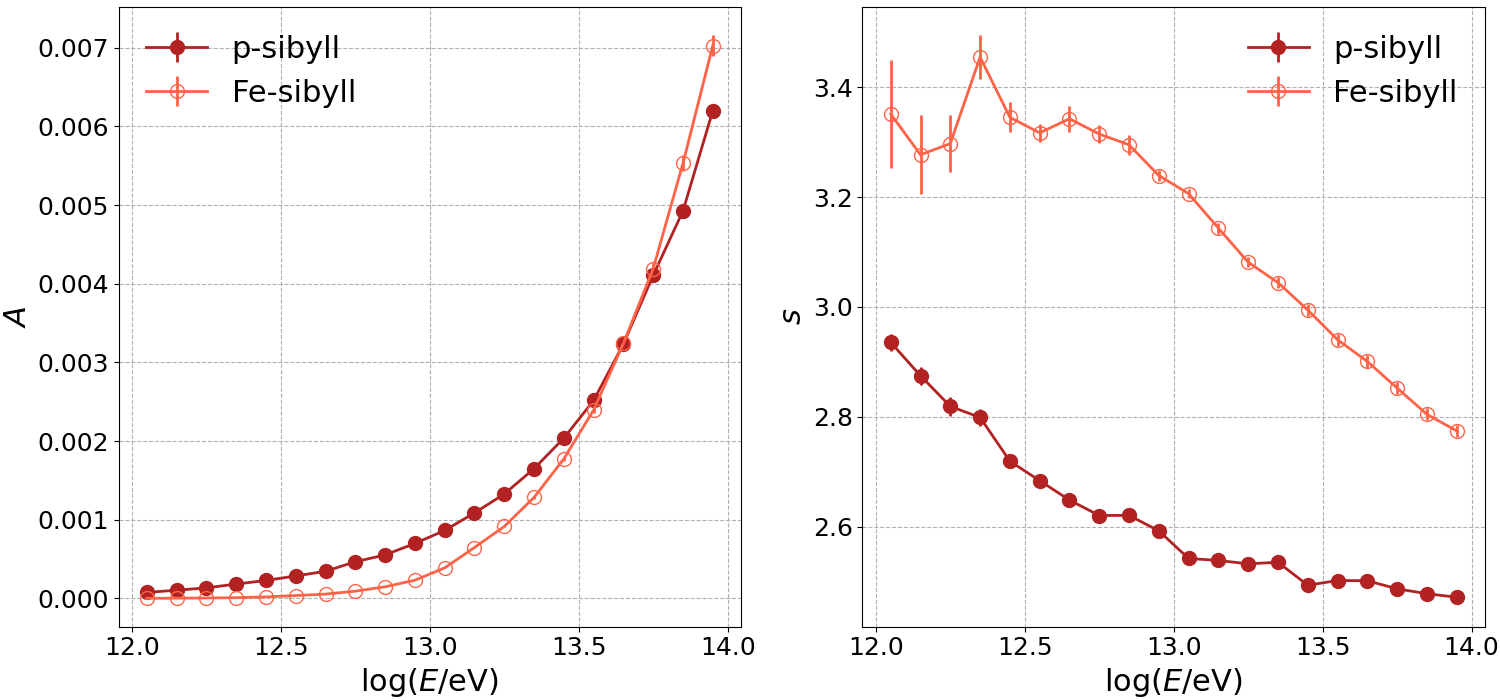
\includegraphics[width=\textwidth]{Figuras/p-composition.png}
\end{frame}

%\begin{frame}{Part\'iculas primarias}
%	\begin{columns}
%		\begin{column}{0.5\textwidth}
%		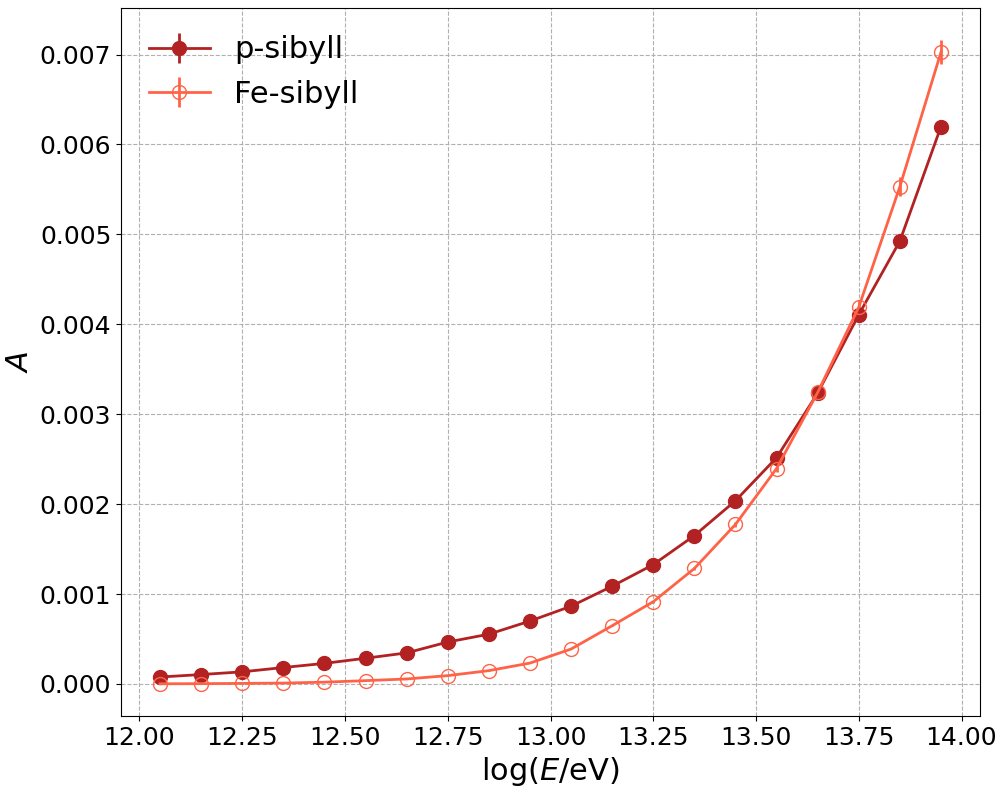
\includegraphics[width=\textwidth]{Figuras/p-composition_nkgA.png}
%		\end{column}
%		
%		\begin{column}{0.5\textwidth}
%		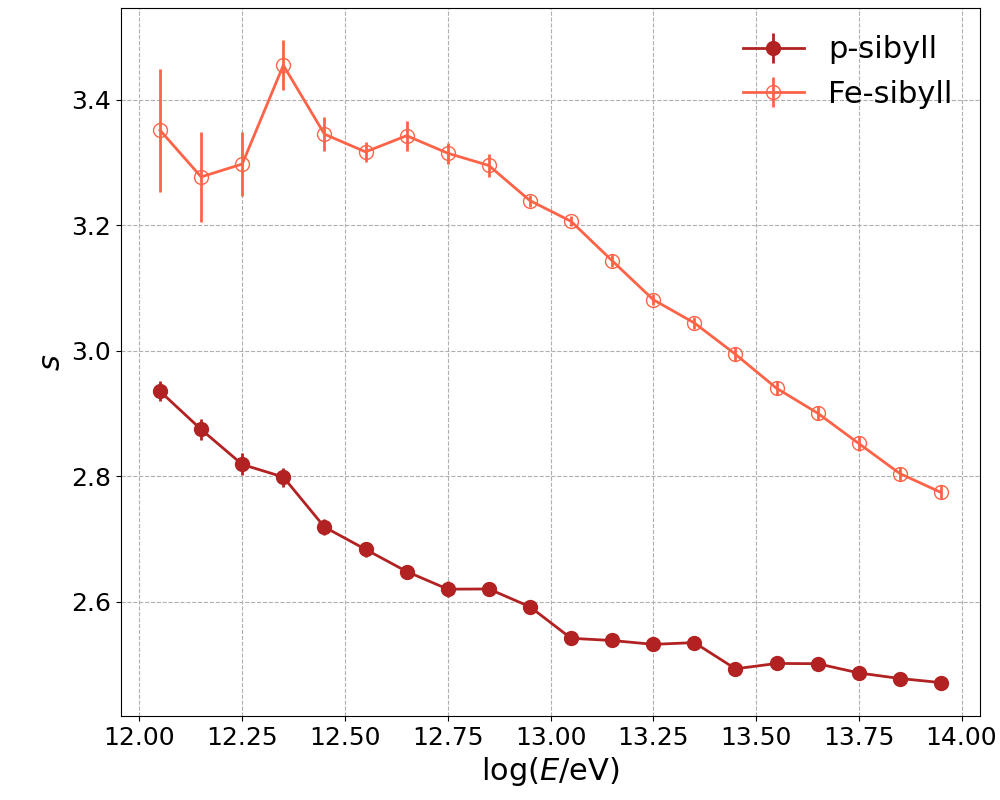
\includegraphics[width=\textwidth]{Figuras/p-composition_nkgs.png}
%		\end{column}
%	\end{columns}
%\end{frame}

%\begin{frame}{\'Angulos de incidencia}
%
%\end{frame}

\begin{frame}{Muones en HAWC}
Se calcul\'o un aproximado del n\'umero de muones que podr\'ian detectarse en un \'area circular de $R=70$ m.
\vspace{0.3cm}
	\begin{center}
	\begin{figure}
	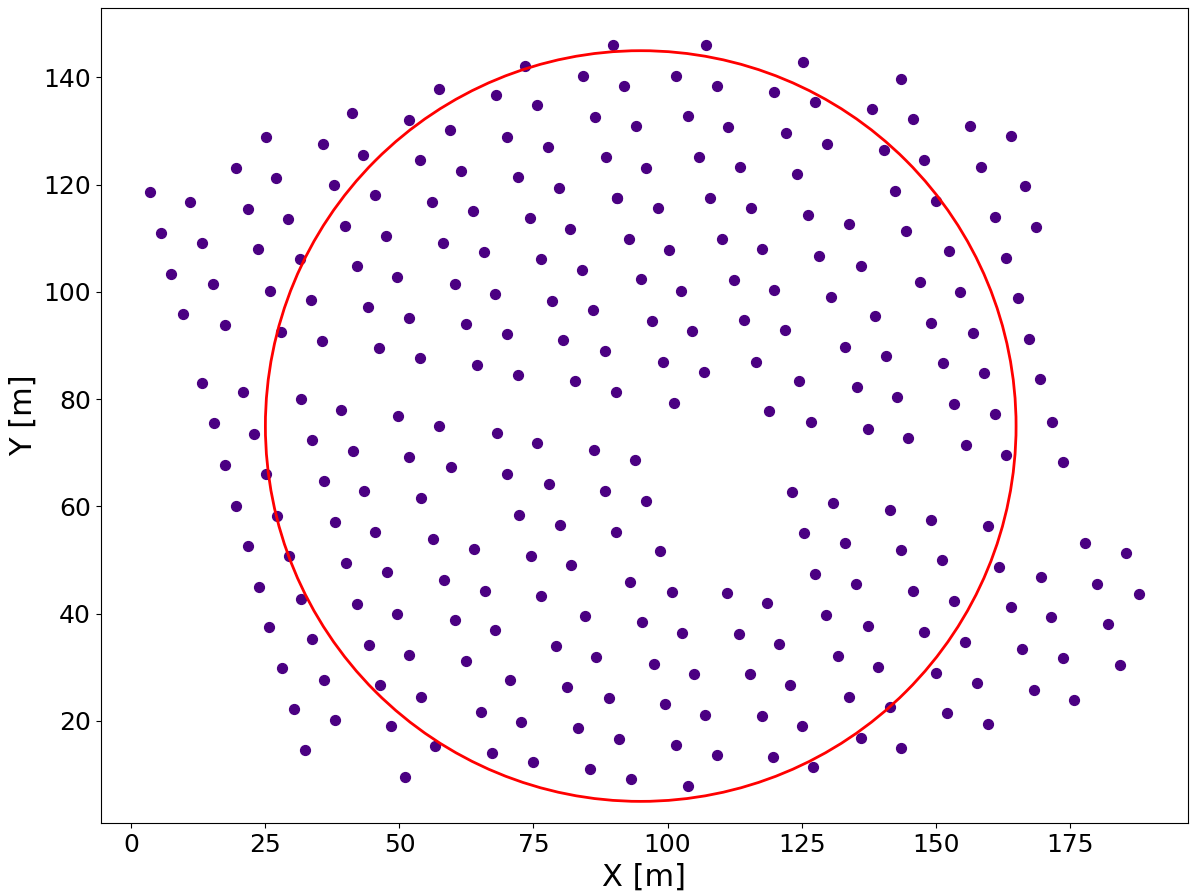
\includegraphics[width=0.7\textwidth]{Figuras/HAWC_array.png}
	\caption{\footnotesize{ Esquema de la disposici\'on de los detectores de agua Cherenkov que conforman HAWC. Cada punto representa un tanque.}}
	\end{figure}
	\end{center}
\end{frame}

\begin{frame}{Muones en HAWC}
\begin{itemize}
\item Se extrajo el n\'umero de muones con $r<70$ m directamente de los resultados de las simulaciones.
\vspace{0.5cm}
\item Independientemente, se calcul\'o el n\'umero de muones a partir de la funci\'on $\rho_{\mu}(r)$ de la forma
	\begin{align*}
	N_{\mu} = 2 \pi \int_0^R r \rho_{\mu}(r) \dd{r},
	\end{align*}
con $R=70$ m.
\end{itemize}
\end{frame}

\begin{frame}{Muones en HAWC}
	\begin{center}
	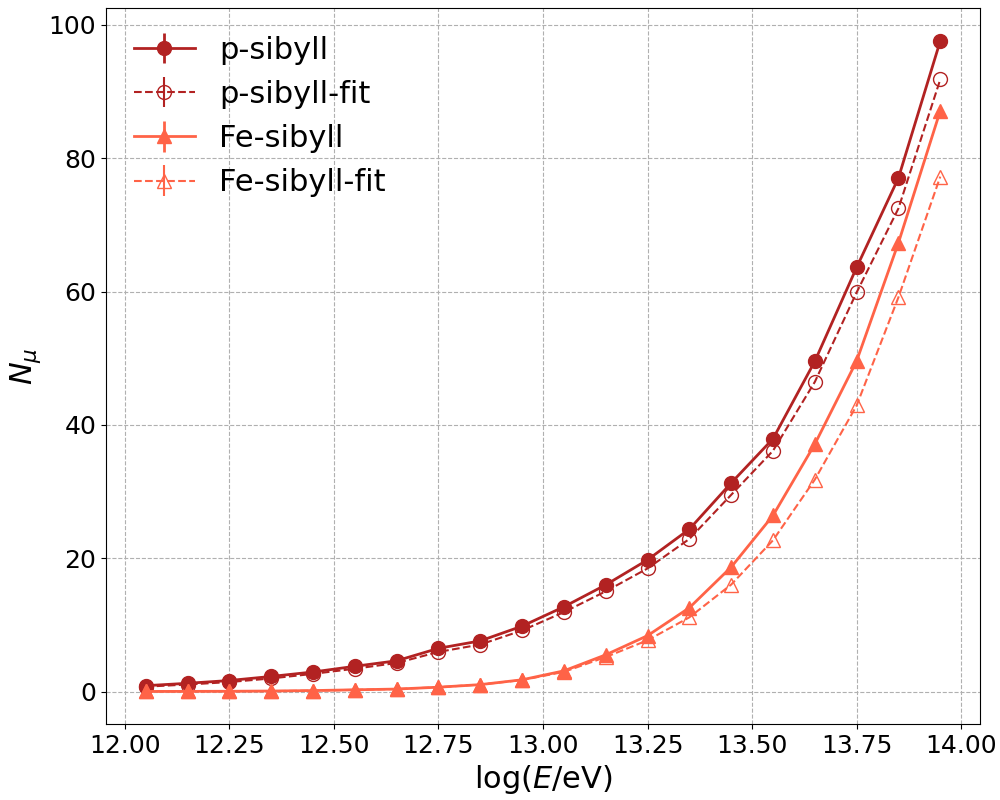
\includegraphics[width=0.9\textwidth]{Figuras/p-munumbers.png}
	\end{center}
\end{frame}


\section{Conclusiones}
\begin{frame}{Conclusiones}
	\begin{itemize}
	\item <+-> En las distancias consideradas ($R<300$ m) se observa que las distribuciones de muones en cascadas de protones est\'an por encima de las de hierro.
	\vspace{0.2cm}
	\item <+-> No se observa una clara dependencia del modelo de interacciones hadr\'onicas en la evoluci\'on de los par\'ametros del ajuste con la energ\'ia primaria.
	\vspace{0.2cm}
	\item <+-> No ser\'ia posible detectar cascadas con energ\'ias menores a $\approx 5$ TeV ya que en un radio de 70 m no se observan suficientes muones.
	\vspace{0.2cm}
	\item <+-> Los ajustes a la funci\'on $\rho_{\mu}(r)$ utilizada en HAWC subestiman $N_{\mu}$ en un promedio del 10\% con respecto a los valores extra\'idos de la simulaci\'on.
	\end{itemize}
	
	\begin{huge}
	\vfill
	\hfill  \onslide<4>\textbf{¡Gracias!}
	\end{huge}
\end{frame}


\end{document}